\documentclass[11pt]{article}

\usepackage[margin=1in]{geometry}
\usepackage{amsmath,amssymb,amsthm,mathtools}
\usepackage{enumitem}
\usepackage{booktabs,longtable,array}
\usepackage{hyperref}
\usepackage{xcolor}
\usepackage{tikz}
\usetikzlibrary{arrows.meta,positioning,fit,calc,shapes.geometric}
\usepackage{graphicx}
\usepackage{listings}
\usepackage{seqsplit}
\usepackage[T1]{fontenc}
\usepackage{lmodern}

\hypersetup{
  colorlinks=true,
  linkcolor=blue!60!black,
  citecolor=blue!60!black,
  urlcolor=blue!60!black
}

\lstset{
  basicstyle=\ttfamily\small,
  columns=fullflexible,
  breaklines=true,
  frame=single,
  framerule=0.3pt,
  rulecolor=\color{black!30},
  backgroundcolor=\color{black!2}
}

\newcommand{\Z}{\mathbb Z}
\newcommand{\N}{\mathbb N}
\newcommand{\R}{\mathbb R}
\newcommand{\PP}{\mathbb P}
\newcommand{\EE}{\mathbb E}
\newcommand{\one}{\mathbf 1}
\newcommand{\conn}{\longleftrightarrow}
\newcommand{\pcrit}{p_c}
\newcommand{\ptilde}{\widetilde p_c}
\newcommand{\Lam}{\Lambda}
\newcommand{\dE}{\partial_E}
\newcommand{\prob}{\operatorname{Prob}}
\newcommand{\supp}{\operatorname{supp}}
\newcommand{\Int}{\operatorname{Int}}
\newcommand{\Ext}{\operatorname{Ext}}
\newcommand{\file}[1]{{\scriptsize\ttfamily\seqsplit{#1}}}

\theoremstyle{definition}
\newtheorem{definition}{Definition}[section]
\newtheorem{task}[definition]{Task}
\newtheorem{interface}[definition]{Lean interface}
\newtheorem{milestone}[definition]{Milestone}

\theoremstyle{plain}
\newtheorem{lemma}[definition]{Lemma}
\newtheorem{theorem}[definition]{Theorem}

\title{Lean Formalization Plan for\\
\emph{A Self-Contained Proof of Sharpness for Nearest-Neighbor Bond Percolation on $\Z^d$}}
\author{Implementation blueprint for Lean 4 + mathlib + Codex}
\date{June 2026}

\begin{document}
\maketitle

\begin{abstract}
This document gives a modular formalization plan for the sharpness proof for nearest-neighbor Bernoulli bond percolation on $\Z^d$.  The plan is designed for a Codex-driven Lean implementation.  The central strategy is to avoid building the infinite product measure at the beginning.  Instead, all probabilities are finite Bernoulli product probabilities attached to finite edge supports, and the infinite-volume quantity $\theta(p)$ is defined as the monotone limit of finite exit probabilities.  The proof is split into geometry, connectivity, finite product probability, independence, Russo's formula, the finite-set criterion, the differential inequality, the supercritical bound, the boundary inequality, subcritical exponential decay, and critical-point identification.
\end{abstract}

\tableofcontents

\section{Target theorem and formalization strategy}

The mathematical target is the following sharpness statement.  Let $d\ge 2$, let vertices be $\Z^d$, and let nearest-neighbor unoriented bonds be open independently with probability $p\in[0,1]$.  Let
\[
  \Lam_n := \{x\in\Z^d : \|x\|_1\le n\},
  \qquad
  a_n(p) := \PP_p(0\conn \Lam_n^c).
\]
Define
\[
  \theta(p) := \lim_{n\to\infty} a_n(p),
  \qquad
  \pcrit := \inf\{p\in[0,1] : \theta(p)>0\}.
\]
The final theorem is:
\begin{enumerate}[label=(\roman*)]
  \item if $p<\pcrit$, then $a_n(p)\le e^{-c n}$ for some $c=c(p)>0$ and every $n$;
  \item if $\pcrit<p<1$, then
  \[
    \theta(p) \ge \frac{p-\pcrit}{p(1-\pcrit)}.
  \]
\end{enumerate}

\subsection{Main Lean design choice: finite-volume probability first}

A direct infinite-product construction is unnecessary for this proof and would make the Lean project much harder.  Instead:
\begin{itemize}[leftmargin=1.4em]
  \item define a global configuration type $\Omega_d := \mathrm{Bond}_d\to\mathrm{Bool}$ only as a semantic object;
  \item define a \emph{local event} as a predicate on $\Omega_d$ together with a finite edge support on which it depends;
  \item define $\PP_p(E)$ for a local event by a finite sum over assignments on its finite support;
  \item define $a_n(p)$ as the finite probability of the local event ``$0$ exits $\Lam_n$'';
  \item define $\theta(p)$ as $\inf_n a_n(p)$, or equivalently as the limit of the decreasing sequence $a_n(p)$.
\end{itemize}
This replacement turns all probabilistic statements in the proof into finite combinatorics plus real analysis.  The only limiting argument needed is monotone convergence of a decreasing sequence of real numbers in $[0,1]$, not measure-theoretic continuity from above for an infinite product measure.

\subsection{Auxiliary finite-set critical point}

For a finite set $S\subset\Z^d$ with $0\in S$, define the oriented edge boundary
\[
  \dE S := \{(x,y): x\in S,\; y\notin S,
        \; \|x-y\|_1=1\},
\]
and
\[
  \varphi_p(S)
  := p\sum_{(x,y)\in\dE S} \PP_p(0\stackrel{S}{\conn}x).
\]
Define
\[
  \ptilde := \sup\{p\in[0,1]:
       \exists \text{ finite }S\ni0\text{ with }\varphi_p(S)<1\}.
\]
The implementation proves the theorem first with $\ptilde$ in place of $\pcrit$, and then proves $\ptilde=\pcrit$.

\section{Recommended Lean file structure}

The project should be built from small files.  Each file should expose theorem statements that later files consume.  Codex should never be asked to prove a late theorem before all earlier interfaces compile.

{\small
\begin{longtable}{p{0.32\textwidth}p{0.37\textwidth}p{0.21\textwidth}}
\toprule
\textbf{Lean file} & \textbf{Contents} & \textbf{Depends on}\\
\midrule
\endfirsthead
\toprule
\textbf{Lean file} & \textbf{Contents} & \textbf{Depends on}\\
\midrule
\endhead
\texttt{Zd}
& Vertices $\Z^d$, $\ell^1$ norm, adjacency, translation, boxes $\Lam_n$.
& mathlib finite sums, integers.\\
\addlinespace
\texttt{Bonds}
& Unoriented nearest-neighbor bonds, canonical bond from adjacent vertices, oriented boundary edges.
& \texttt{Zd}.\\
\addlinespace
\texttt{FiniteGeometry}
& Finite internal edge sets, exit edge supports, boundary endpoint bounds, $\ell^1$ triangle arguments.
& \texttt{Zd}, \texttt{Bonds}.\\
\addlinespace
\texttt{Paths}
& Lists as paths, path concatenation, first/last exit lemmas, connectivity inside a finite set.
& \texttt{Bonds}, \texttt{FiniteGeometry}.\\
\addlinespace
\texttt{Clusters}
& Finite cluster $C_S(u)$, cluster event $C_S(u)=C_0$, cluster-boundary facts.
& \texttt{Paths}.\\
\addlinespace
\texttt{FiniteBernoulli}
& Finite Bernoulli product probability by finite sums, total mass, complement, union bound.
& mathlib algebra and finite sums.\\
\addlinespace
\texttt{LocalEvent}
& Local events, finite supports, support extension invariance, event operations.
& \texttt{FiniteBernoulli}, \texttt{Bonds}.\\
\addlinespace
\texttt{Independence}
& Disjoint-support multiplication and finite independence for two and three local events.
& \texttt{LocalEvent}.\\
\addlinespace
\texttt{Monotonicity}
& Increasing events, monotonicity of $p\mapsto\PP_p(E)$, monotonicity of $\varphi_p(S)$.
& \texttt{LocalEvent}.\\
\addlinespace
\texttt{Russo}
& Closed-pivotal Russo formula for finite local increasing events.
& \texttt{LocalEvent}, \texttt{Independence}, calculus.\\
\addlinespace
\texttt{Events}
& Local events $x\stackrel{S}{\conn}y$, $x\conn\Lam_n^c$, finite exit event $A_\Lam$.
& \texttt{Paths}, \texttt{LocalEvent}.\\
\addlinespace
\texttt{Phi}
& $\varphi_p(S)$, $\ptilde$, elementary consequences of the supremum definition.
& \texttt{Events}, \texttt{Monotonicity}.\\
\addlinespace
\texttt{DiffIneq}
& Lemma 2: fundamental differential inequality.
& \texttt{Russo}, \texttt{Phi}, \texttt{Events}.\\
\addlinespace
\texttt{OdeComparison}
& Generic calculus lemma integrating $f'\ge(1-f)/(p(1-p))$.
& real calculus.\\
\addlinespace
\texttt{Supercritical}
& Lemma 3: lower bound above $\ptilde$.
& \texttt{DifferentialInequality}, \texttt{OdeComparison}.\\
\addlinespace
\texttt{BoundaryIneq}
& Lemma 4: finite-set expansion inequality.
& \texttt{Clusters}, \texttt{Independence}.\\
\addlinespace
\texttt{Subcritical}
& Lemma 5: exponential decay below $\ptilde$.
& \texttt{BoundaryInequality}, \texttt{Phi}, \texttt{FiniteGeometry}.\\
\addlinespace
\texttt{CriticalPoint}
& Definition of $\theta$, $\pcrit$, proof $\ptilde=\pcrit$.
& \texttt{Supercritical}, \texttt{Subcritical}.\\
\addlinespace
\texttt{Main}
& Final theorem with $\pcrit$.
& \texttt{CriticalPoint}.\\
\bottomrule
\end{longtable}
}

\section{Fact graph}

The following graph is the dependency skeleton.  A solid arrow means a theorem directly uses the previous block.  The large boxes show the three foundations: geometry/connectivity, finite probability, and real-order/calculus.

\begin{center}
\resizebox{\textwidth}{!}{%
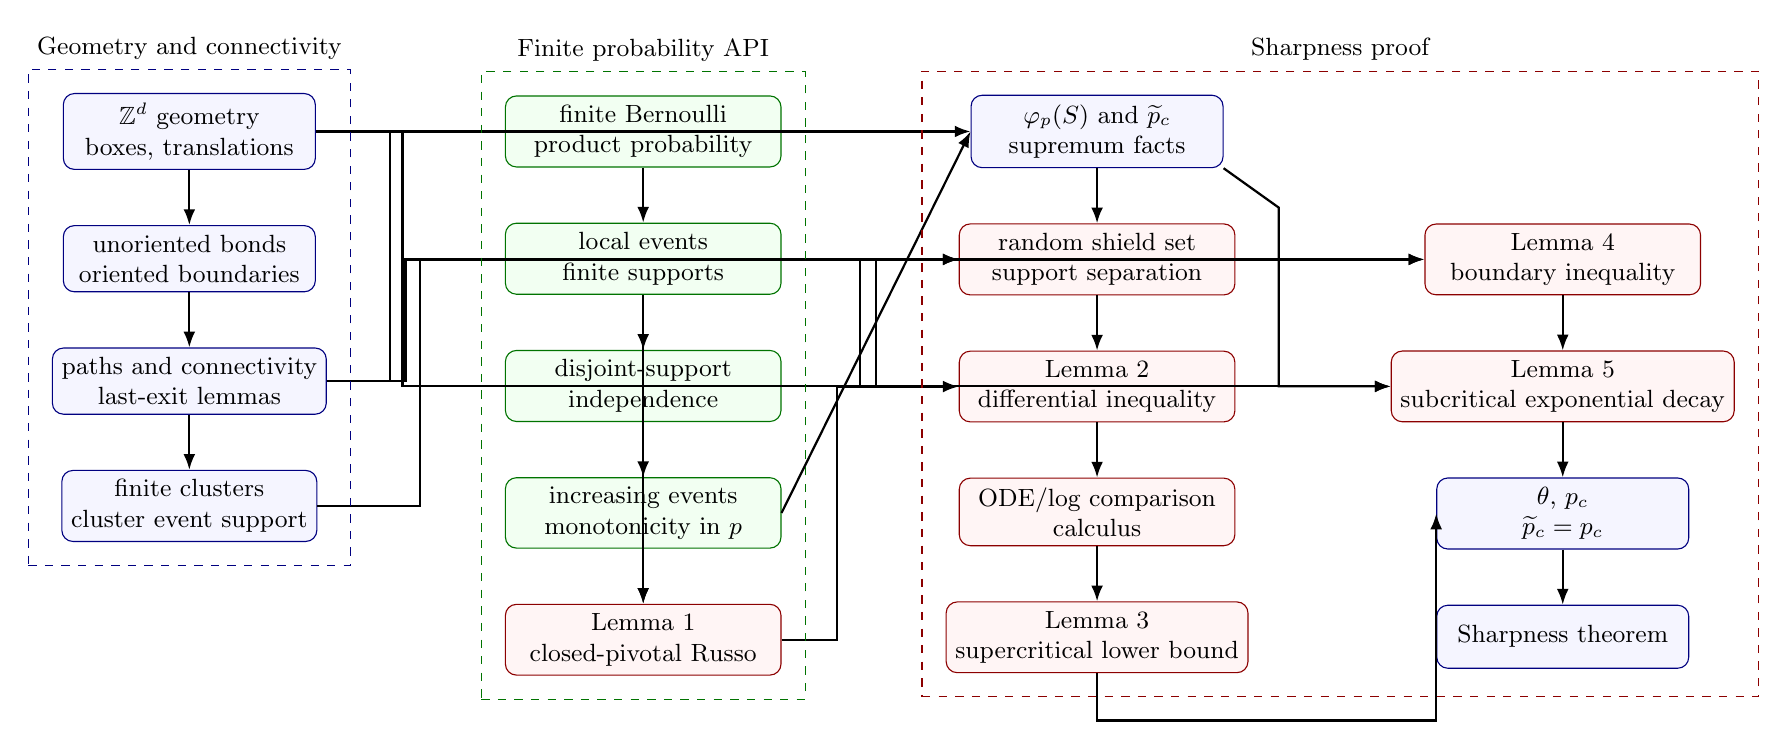
\begin{tikzpicture}[
  node distance=7mm and 12mm,
  fact/.style={rectangle, rounded corners, draw=blue!50!black, fill=blue!4, align=center, minimum width=32mm, minimum height=8mm, font=\small},
  hard/.style={rectangle, rounded corners, draw=red!55!black, fill=red!4, align=center, minimum width=35mm, minimum height=8mm, font=\small},
  prob/.style={rectangle, rounded corners, draw=green!45!black, fill=green!5, align=center, minimum width=35mm, minimum height=8mm, font=\small},
  arr/.style={-{Latex[length=2mm]}, thick}
]

\node[fact] (zd) {$\Z^d$ geometry\\boxes, translations};
\node[fact, below=of zd] (bonds) {unoriented bonds\\oriented boundaries};
\node[fact, below=of bonds] (paths) {paths and connectivity\\last-exit lemmas};
\node[fact, below=of paths] (clusters) {finite clusters\\cluster event support};

\node[prob, right=24mm of zd] (bern) {finite Bernoulli\\product probability};
\node[prob, below=of bern] (local) {local events\\finite supports};
\node[prob, below=of local] (indep) {disjoint-support\\independence};
\node[prob, below=of indep] (mono) {increasing events\\monotonicity in $p$};
\node[hard, below=of mono] (russo) {Lemma 1\\closed-pivotal Russo};

\node[fact, right=24mm of bern] (phi) {$\varphi_p(S)$ and $\ptilde$\\supremum facts};
\node[hard, below=of phi] (shield) {random shield set\\support separation};
\node[hard, below=of shield] (diff) {Lemma 2\\differential inequality};
\node[hard, below=of diff] (ode) {ODE/log comparison\\calculus};
\node[hard, below=of ode] (super) {Lemma 3\\supercritical lower bound};

\node[hard, right=24mm of shield] (boundary) {Lemma 4\\boundary inequality};
\node[hard, below=of boundary] (subcrit) {Lemma 5\\subcritical exponential decay};
\node[fact, below=of subcrit] (crit) {$\theta$, $\pcrit$\\$\ptilde=\pcrit$};
\node[fact, below=of crit] (main) {Sharpness theorem};

\draw[arr] (zd) -- (bonds);
\draw[arr] (bonds) -- (paths);
\draw[arr] (paths) -- (clusters);
\draw[arr] (bern) -- (local);
\draw[arr] (local) -- (indep);
\draw[arr] (local) -- (mono);
\draw[arr] (mono) -- (russo);
\draw[arr] (indep) -- (russo);
\draw[arr] (paths.east) -- ++(8mm,0) |- (phi.west);
\draw[arr] (mono.east) -- (phi.west);
\draw[arr] (phi) -- (shield);
\draw[arr] (indep.east) -- ++(10mm,0) |- (shield.west);
\draw[arr] (paths.east) -- ++(10mm,0) |- (shield.west);
\draw[arr] (russo.east) -- ++(7mm,0) |- (diff.west);
\draw[arr] (shield) -- (diff);
\draw[arr] (diff) -- (ode);
\draw[arr] (ode) -- (super);
\draw[arr] (clusters.east) -- ++(13mm,0) |- (boundary.west);
\draw[arr] (indep.east) -- ++(12mm,0) |- (boundary.west);
\draw[arr] (phi.south east) -- ++(7mm,-5mm) |- (subcrit.west);
\draw[arr] (boundary) -- (subcrit);
\draw[arr] (zd.east) -- ++(11mm,0) |- (subcrit.west);
\draw[arr] (super.south) -- ++(0,-6mm) -| (crit.west);
\draw[arr] (subcrit) -- (crit);
\draw[arr] (crit) -- (main);

\node[draw=blue!50!black, dashed, fit=(zd)(bonds)(paths)(clusters), inner sep=3mm, label={[font=\small]above:Geometry and connectivity}] {};
\node[draw=green!45!black, dashed, fit=(bern)(local)(indep)(mono)(russo), inner sep=3mm, label={[font=\small]above:Finite probability API}] {};
\node[draw=red!55!black, dashed, fit=(phi)(shield)(diff)(ode)(super)(boundary)(subcrit)(crit)(main), inner sep=3mm, label={[font=\small]above:Sharpness proof}] {};
\end{tikzpicture}%
}
\end{center}

\section{Part I: $\Z^d$ geometry and bonds}

\subsection{Vertices, norm, adjacency, and boxes}

Use
\[
  \mathrm{Vertex}(d) := \mathrm{Fin}(d)\to\Z.
\]
Define
\[
  \|x\|_1 := \sum_{i:\mathrm{Fin}(d)} |x_i|,
  \qquad
  x\sim y \iff \|x-y\|_1=1.
\]
Define $\Lam_n$ as a \texttt{Finset} by filtering the finite product box $[-n,n]^d$ by the condition $\|x\|_1\le n$.  Avoid using an infinite set plus a separate finiteness proof whenever possible.

\begin{interface}[core geometry statements]
The following are the Lean-level facts needed later.
\begin{lstlisting}
def Vertex (d : Nat) := Fin d -> Int

def l1 (x : Vertex d) : Nat := ...
def Adj (x y : Vertex d) : Prop := l1 (x - y) = 1

def ball (d : Nat) (n : Nat) : Finset (Vertex d) := ...

lemma mem_ball_iff : x in ball d n <-> l1 x <= n
lemma zero_mem_ball : (0 : Vertex d) in ball d n
lemma adj_l1_triangle : Adj x y -> l1 z <= n -> ...
lemma translate_ball_exit :
  y in ball d L -> z notin ball d n -> z - y notin ball d (n - L)

def translateVertex (a x : Vertex d) : Vertex d := x + a
lemma adj_translate_iff : Adj (x+a) (y+a) <-> Adj x y
\end{lstlisting}
\end{interface}

The key geometric lemma for subcritical decay is:
\begin{lemma}[translation-to-origin estimate]
If $y\in\Lam_L$ and $z\notin\Lam_n$, then $z-y\notin\Lam_{n-L}$ for $n\ge L$.  Equivalently, any path from $y$ to $\Lam_n^c$ translates to a path from $0$ to $\Lam_{n-L}^c$.
\end{lemma}
\begin{proof}[Proof idea]
Use the $\ell^1$ triangle inequality:
\[
  \|z-y\|_1 \ge \|z\|_1-\|y\|_1 > n-L.
\]
In Lean it is often easier to prove the contrapositive using natural-valued inequalities:
$\|z-y\|_1\le n-L$ and $\|y\|_1\le L$ imply $\|z\|_1\le n$.
\end{proof}

\subsection{Unoriented bonds and oriented boundaries}

The percolation state should live on unoriented bonds.  Boundary sums, however, are naturally over oriented pairs $(x,y)$ with $x\in S$, $y\notin S$.  Recommended design:
\begin{itemize}[leftmargin=1.4em]
  \item define an unoriented bond as a two-element finite set of adjacent vertices, or as a canonical sorted pair;
  \item define \texttt{bondOfAdj x y} for adjacent vertices;
  \item define oriented boundary edges as vertex pairs, with a projection to the associated unoriented bond.
\end{itemize}

\begin{interface}[bonds and boundaries]
\begin{lstlisting}
structure Bond (d : Nat) where
  carrier : Finset (Vertex d)
  card_two : carrier.card = 2
  adj_pair : forall x in carrier, forall y in carrier,
    x != y -> Adj x y

def bondOfAdj (hxy : Adj x y) : Bond d := ...

structure OEdgeBoundary (S : Finset (Vertex d)) where
  x : Vertex d
  y : Vertex d
  hx : x in S
  hy : y notin S
  hxy : Adj x y

def OEdgeBoundary.bond (e : OEdgeBoundary S) : Bond d := bondOfAdj e.hxy

def internalBonds (S : Finset (Vertex d)) : Finset (Bond d) := ...
def exitBonds (S : Finset (Vertex d)) : Finset (Bond d) := ...
\end{lstlisting}
\end{interface}

The most important support-disjointness facts are:
\begin{align*}
  \Int(S) &:= \{\{x,y\}: x,y\in S,\ x\sim y\},\\
  \Ext(S) &:= \text{finite ambient support}\setminus \Int(S),\\
  \Int(S)\cap \Ext(S) &= \varnothing.
\end{align*}
For Lemma 4, also define
\[
  E(S,C_0) := \{\{a,b\}: a,b\in S,\ \{a,b\}\cap C_0\ne\varnothing\}.
\]
Then $E(S,C_0)$ is disjoint from a boundary edge $xy$ with $x\in C_0$, $y\notin S$, and from the edges used by paths in $\Z^d\setminus C_0$.

\section{Part II: paths, connectivity, and clusters}

\subsection{Paths}

Represent paths by lists of vertices.  A path is valid if consecutive vertices are adjacent.  It is open in a configuration if every consecutive bond is open.  It stays in $S$ if every vertex of the list belongs to $S$.

\begin{interface}[path and connectivity definitions]
\begin{lstlisting}
def IsPath (gamma : List (Vertex d)) : Prop := ...
def PathFromTo (gamma : List (Vertex d)) (x y : Vertex d) : Prop := ...
def PathIn (S : Finset (Vertex d)) (gamma : List (Vertex d)) : Prop := ...
def OpenPath (omega : Config d) (gamma : List (Vertex d)) : Prop := ...

def ConnIn (omega : Config d) (S : Finset (Vertex d))
    (x y : Vertex d) : Prop :=
  exists gamma, PathFromTo gamma x y and PathIn S gamma and OpenPath omega gamma
\end{lstlisting}
\end{interface}

Do not initially try to build a sophisticated graph library.  The proof only needs path reversal, path concatenation, translation of paths, and last-exit facts for finite lists.

\subsection{Finite exit event}

For a finite $\Lam\ni0$, define the finite exit event $A_\Lam$ by first reducing the informal event $\{0\conn\Lam^c\}$ to a boundary-crossing event.  Namely,
\[
  A_\Lam(\omega) \iff
  \exists (x,y)\in\dE\Lam,
       0\stackrel{\Lam}{\conn}x
       \text{ and } \omega(\{x,y\})=\mathrm{open}.
\]
Thus $A_\Lam$ is a local event supported on internal bonds of $\Lam$ plus boundary bonds of $\Lam$.

\begin{interface}[finite exit event]
\begin{lstlisting}
def ExitEvent (Lam : Finset (Vertex d)) (h0 : 0 in Lam) : LocalEvent d := ...
def exitProb (p : Real) (Lam : Finset (Vertex d)) : Real :=
  Prob p (ExitEvent Lam h0)

def boxExitProb (p : Real) (n : Nat) : Real :=
  exitProb p (ball d n)
\end{lstlisting}
\end{interface}

This definition replaces the infinite event $\{0\conn\Lam^c\}$ everywhere.  It is mathematically equivalent for nearest-neighbor finite $\Lam$ because an exit path has a first edge leaving $\Lam$.

\subsection{Clusters inside a finite set}

For Lemma 4 define
\[
  C_S(u;\omega):=\{x\in S:u\stackrel S\conn x\}.
\]
The event $C_S(u)=C_0$ is local.  Its minimal support is not all of $\Int(S)$; it suffices to use the bonds inside $S$ with at least one endpoint in $C_0$.  This sharper support statement is useful for independence.

\begin{lemma}[cluster event support]
On the event $C_S(u)=C_0$, whether the event holds is determined by the states of bonds $\{a,b\}$ with $a,b\in S$ and at least one endpoint in $C_0$.
\end{lemma}
\begin{proof}[Proof idea]
To know $C_S(u)=C_0$, it is enough to know that all vertices of $C_0$ are connected to $u$ inside $C_0$ using open bonds, and all boundary bonds from $C_0$ to $S\setminus C_0$ are closed.  Edges wholly inside $S\setminus C_0$ cannot change the cluster of $u$.
\end{proof}

\section{Part III: finite Bernoulli product probability}

\subsection{Finite product probability by sums}

For a finite edge set $F$, let $\{0,1\}^F$ be assignments of open/closed states.  Define
\[
  w_p(\sigma):=\prod_{e\in F}
       \begin{cases}
       p,&\sigma(e)=1,\\
       1-p,&\sigma(e)=0,
       \end{cases}
\]
and
\[
  \prob_p^F(A):=\sum_{\sigma\in\{0,1\}^F}\one_A(\sigma)w_p(\sigma).
\]
Use real-valued probabilities, not \texttt{ENNReal}, because Russo's formula and the supercritical integration are real-calculus statements.

\begin{interface}[finite Bernoulli probability]
\begin{lstlisting}
def weight (p : Real) (F : Finset (Bond d)) (sigma : F -> Bool) : Real := ...
def ProbOn (p : Real) (F : Finset (Bond d)) (A : (F -> Bool) -> Prop) : Real :=
  sum sigma, if A sigma then weight p F sigma else 0

lemma prob_nonneg (hp0 : 0 <= p) (hp1 : p <= 1) : 0 <= ProbOn p F A
lemma prob_le_one (hp0 : 0 <= p) (hp1 : p <= 1) : ProbOn p F A <= 1
lemma prob_univ (hp0 : 0 <= p) (hp1 : p <= 1) : ProbOn p F True = 1
lemma prob_compl : ProbOn p F (not A) = 1 - ProbOn p F A
lemma prob_union_bound : ProbOn p F (A or B) <= ProbOn p F A + ProbOn p F B
\end{lstlisting}
\end{interface}

\subsection{Local events and support extension}

To avoid changing probability spaces constantly, wrap local predicates as predicates on global configurations plus a finite support.

\begin{interface}[local events]
\begin{lstlisting}
abbrev Config (d : Nat) := Bond d -> Bool

def DependsOn (F : Finset (Bond d)) (A : Config d -> Prop) : Prop :=
  forall omega omega', (forall e in F, omega e = omega' e) -> (A omega <-> A omega')

structure LocalEvent (d : Nat) where
  support : Finset (Bond d)
  pred : Config d -> Prop
  local : DependsOn support pred

def Prob (p : Real) (E : LocalEvent d) : Real := ...
\end{lstlisting}
\end{interface}

Essential support lemmas:
\begin{enumerate}[label=(S\arabic*)]
  \item If $E$ depends on $F$ and $F\subset G$, then computing $\PP_p(E)$ using $F$ or $G$ gives the same number.
  \item $E\cap E'$, $E\cup E'$, and $E^c$ are local, with support contained in the union of supports.
  \item If $E$ and $E'$ have disjoint supports, then $\PP_p(E\cap E')=\PP_p(E)\PP_p(E')$.
  \item The same multiplication lemma should be available for three events with pairwise disjoint supports.
\end{enumerate}

\subsection{Independence API}

The independence lemmas are used in only two places: Lemma 2 and Lemma 4.  A specialized disjoint-support theorem is enough.

\begin{lemma}[disjoint-support independence]
Let $E_1,E_2$ be local events with disjoint supports.  For $0\le p\le1$,
\[
  \PP_p(E_1\cap E_2)=\PP_p(E_1)\PP_p(E_2).
\]
If $E_1,E_2,E_3$ have pairwise disjoint supports, then
\[
  \PP_p(E_1\cap E_2\cap E_3)
  =\PP_p(E_1)\PP_p(E_2)\PP_p(E_3).
\]
\end{lemma}
\begin{proof}[Proof idea]
Reduce to finite products over $F_1\cup F_2$ or $F_1\cup F_2\cup F_3$ and use factorization of finite sums over product types.  This is purely finite algebra.
\end{proof}

\subsection{Monotonicity in $p$}

The definition of $\ptilde$ uses monotonicity of $\varphi_p(S)$.  Prove monotonicity of probabilities of increasing local events once.

\begin{definition}[increasing local event]
A local event $E$ is increasing if $\omega\le\omega'$ coordinatewise and $E(\omega)$ imply $E(\omega')$.
\end{definition}

\begin{lemma}[Bernoulli monotonicity]
If $E$ is increasing and $0\le p\le q\le1$, then
\[
  \PP_p(E)\le\PP_q(E).
\]
\end{lemma}
\begin{proof}[Proof idea]
Use the standard coupling: give each edge an independent uniform variable in a finite ordered grid, or prove directly by induction on the finite support.  The induction proof is usually easier in Lean: condition on one edge and use
\[
  \PP_p(E)=(1-p)\PP_p(E|e=0)+p\PP_p(E|e=1),
\]
with $\PP_p(E|e=0)\le\PP_p(E|e=1)$ for increasing $E$.
\end{proof}

Then $p\mapsto\varphi_p(S)$ is nondecreasing because it is a finite sum of products of $p$ and increasing connection probabilities.

\section{Part IV: Russo's formula}

\subsection{Closed-pivotal form}

For a local increasing event $A$ and an edge $e$ in its support, define ``$e$ is closed-pivotal'' as:
\begin{itemize}[leftmargin=1.4em]
  \item $e$ is closed;
  \item $A$ does not occur;
  \item after forcing $e$ to be open, $A$ occurs.
\end{itemize}

\begin{theorem}[Lemma 1, Russo closed-pivotal form]
If $A$ is increasing and local, then for $0<p<1$,
\[
  \frac{d}{dp}\PP_p(A)
  =\frac{1}{1-p}\sum_{e\in\supp(A)}
     \PP_p(e\text{ is closed-pivotal for }A).
\]
\end{theorem}

\subsection{Lean proof plan for Russo}

Implement Russo in a generic finite Boolean product file, independent of percolation.

\begin{enumerate}[leftmargin=1.4em]
  \item For an event $A\subseteq\{0,1\}^F$, define the edge-influence event $B_e$ on $F\setminus\{e\}$: changing $e$ changes $A$.
  \item Prove the single-coordinate derivative identity
  \[
    \frac{\partial}{\partial p_e}\PP_{(p_f)}(A)=\PP_{(p_f)_{f\ne e}}(B_e).
  \]
  \item Specialize to the homogeneous case $p_f=p$ and sum over $e\in F$.
  \item For increasing $A$, prove
  \[
    \PP_p(e\text{ closed-pivotal})=(1-p)\PP_p(B_e).
  \]
\end{enumerate}

The most Codex-friendly route is an induction on the finite list of edges, not a high-level measure-theory proof.  Keep all differentiability statements in $\R$.

\begin{interface}[Russo theorem stub]
\begin{lstlisting}
theorem russo_closed_pivotal
  (E : LocalEvent d) (hinc : Increasing E)
  {p : Real} (hp0 : 0 < p) (hp1 : p < 1) :
  HasDerivAt (fun q => Prob q E)
    ((1 / (1 - p)) * sum e in E.support, Prob p (closedPivotalEvent E e)) p := ...
\end{lstlisting}
\end{interface}

\section{Part V: the finite-set criterion $\varphi_p(S)$ and $\ptilde$}

\subsection{Definition of $\varphi_p(S)$}

For finite $S\ni0$,
\[
  \varphi_p(S)=p\sum_{(x,y)\in\dE S}\PP_p(0\stackrel S\conn x).
\]
The event $0\stackrel S\conn x$ is local with support $\Int(S)$.

\begin{interface}[phi and p-tilde]
\begin{lstlisting}
def phi (p : Real) (S : Finset (Vertex d)) : Real :=
  p * sum e in orientedBoundary S, Prob p (connInEvent S 0 e.x)

def pTilde : Real :=
  sSup {p : Real | 0 <= p and p <= 1 and exists S, finite S and 0 in S and phi p S < 1}
\end{lstlisting}
\end{interface}

\subsection{Order consequences}

Prove the two consequences as standalone order lemmas.

\begin{lemma}[below $\ptilde$]
If $p<\ptilde$, then there exists a finite $S\ni0$ such that $\varphi_p(S)<1$.
\end{lemma}
\begin{proof}[Proof idea]
By the definition of supremum, choose $q>p$ in the set.  Then choose $S$ with $\varphi_q(S)<1$.  Monotonicity gives $\varphi_p(S)\le\varphi_q(S)<1$.
\end{proof}

\begin{lemma}[above $\ptilde$]
If $p>\ptilde$, then for every finite $S\ni0$, $\varphi_p(S)\ge1$.
\end{lemma}
\begin{proof}[Proof idea]
Otherwise $p$ itself belongs to the set defining $\ptilde$, contradicting $p>\sup$.
\end{proof}

These two lemmas are repeatedly used and should not be reproved inside later files.

\section{Part VI: Lemma 2, the fundamental differential inequality}

\subsection{Statement}

For finite $\Lam\ni0$, define $f_\Lam(p):=\PP_p(A_\Lam)$.  Lemma 2 states:
\[
  f_\Lam'(p)
  \ge
  \frac{1}{p(1-p)}
  \inf_{\substack{S\subset\Lam\\0\in S}}
  \varphi_p(S)\,(1-f_\Lam(p)).
\]
In Lean, since the infimum is over finitely many subsets of $\Lam$, use a finite minimum rather than a set-theoretic infimum.

\begin{interface}[finite minimum version]
\begin{lstlisting}
def phiMinIn (p : Real) (Lam : Finset (Vertex d)) : Real :=
  Finset.inf' {S : Finset (Vertex d) | S subset Lam and 0 in S} ... (phi p S)

theorem differential_inequality
  (Lam : Finset (Vertex d)) (h0 : 0 in Lam)
  {p : Real} (hp0 : 0 < p) (hp1 : p < 1) :
  deriv (fun q => exitProb q Lam) p >=
    (1 / (p * (1 - p))) * phiMinIn p Lam * (1 - exitProb p Lam) := ...
\end{lstlisting}
\end{interface}

\subsection{The random shield set}

Define
\[
  \mathcal S(\omega):=
  \{x\in\Lam : x\not\conn\Lam^c\}.
\]
In the finite formalization, $x\conn\Lam^c$ means the finite exit event from $x$ through $\dE\Lam$.
Then
\[
  0\in\mathcal S(\omega) \iff A_\Lam(\omega)^c.
\]

\begin{lemma}[support separation for $\{\mathcal S=S\}$]
Fix $S\subset\Lam$.  The event $\{\mathcal S=S\}$ is determined by the edge states not internal to $S$.
\end{lemma}
\begin{proof}[Proof idea]
Delete all internal edges of $S$.  Then $\{\mathcal S=S\}$ is equivalent to:
\begin{enumerate}[label=(\alph*)]
  \item no vertex of $S$ is connected to $\Lam^c$ in the deleted-internal-edge graph;
  \item every vertex of $\Lam\setminus S$ is connected to $\Lam^c$ in the deleted-internal-edge graph.
\end{enumerate}
Both conditions use only non-internal edges.  The nontrivial direction is a last-exit argument: if a path using internal $S$-edges connects a vertex of $S$ to $\Lam^c$, take the last exit from $S$; the tail witnesses a connection to $\Lam^c$ without internal $S$-edges.  The same argument handles vertices of $\Lam\setminus S$.
\end{proof}

\subsection{Pivotal equivalence}

Fix $S\subset\Lam$ with $0\in S$ and an oriented boundary edge $(x,y)\in\dE S$.  On $\{\mathcal S=S\}$,
\[
  \{xy\text{ is closed-pivotal for }A_\Lam\}
  \iff
  \{0\stackrel S\conn x\}.
\]
The edge $xy$ is automatically closed on the right-hand side; otherwise $x$ would connect to $\Lam^c$, contradicting $x\in\mathcal S$.

\subsection{Differential inequality proof chain}

The formal proof should follow this exact chain.
\begin{enumerate}[leftmargin=1.4em]
  \item Apply Russo to $A_\Lam$:
  \[
    f_\Lam'(p)=\frac1{1-p}\sum_e \PP_p(e\text{ closed-pivotal}).
  \]
  \item Decompose by values of $\mathcal S$ with $0\in S$.
  \item Restrict the sum to closed-pivotal edges oriented from $S$ to $S^c$.
  \item Use pivotal equivalence:
  \[
    \PP_p(e\text{ closed-pivotal},\mathcal S=S)
    =\PP_p(0\stackrel S\conn x,\mathcal S=S).
  \]
  \item Use support separation and disjoint-support independence:
  \[
    \PP_p(0\stackrel S\conn x,\mathcal S=S)
    =\PP_p(0\stackrel S\conn x)\PP_p(\mathcal S=S).
  \]
  \item Sum over $(x,y)\in\dE S$ and use the definition of $\varphi_p(S)$:
  \[
    \sum_{(x,y)\in\dE S}
    \PP_p(0\stackrel S\conn x)\PP_p(\mathcal S=S)
    =\frac{\varphi_p(S)}{p}\PP_p(\mathcal S=S).
  \]
  \item Bound $\varphi_p(S)$ below by the finite minimum over $S\subset\Lam$, $0\in S$.
  \item Sum $\PP_p(\mathcal S=S)$ over all $S\subset\Lam$ with $0\in S$, obtaining
  \[
    \PP_p(0\in\mathcal S)=1-f_\Lam(p).
  \]
\end{enumerate}

This is one of the two hardest mathematical modules.  The recommended Codex workflow is: first formalize the statement with the support-separation and pivotal-equivalence lemmas as named hypotheses; then prove those two lemmas separately.

\section{Part VII: Lemma 3, supercritical lower bound}

\subsection{Generic calculus lemma}

Isolate the real-analysis step.

\begin{lemma}[ODE/log comparison]
Let $0<q<p<1$.  Suppose $f:[q,p]\to\R$ is differentiable, $f(t)<1$, and
\[
  f'(t)\ge \frac{1-f(t)}{t(1-t)}
  \qquad (q<t<p).
\]
Then
\[
  1-f(p)
  \le
  (1-f(q))\frac{q(1-p)}{p(1-q)}.
\]
\end{lemma}
\begin{proof}[Proof idea]
Apply the derivative identity
\[
  \frac{d}{dt}\log(1-f(t))=-\frac{f'(t)}{1-f(t)}
\]
and integrate:
\[
  \log\frac{1-f(p)}{1-f(q)}
  \le
  -\int_q^p\frac{dt}{t(1-t)}
  =-\log\frac{p(1-q)}{q(1-p)}.
\]
The side condition $f(t)<1$ follows for finite exit events by closing all boundary edges of $\Lam$.
\end{proof}

\subsection{Supercritical proof chain}

For $\ptilde<p<1$:
\begin{enumerate}[leftmargin=1.4em]
  \item Fix finite $\Lam\ni0$.
  \item For every $q>\ptilde$, the order lemma gives $\varphi_q(S)\ge1$ for all finite $S\ni0$.
  \item Lemma 2 gives
  \[
    f_\Lam'(q)
    \ge \frac{1}{q(1-q)}(1-f_\Lam(q)).
  \]
  \item Apply ODE/log comparison from $q$ to $p$.
  \item Use $1-f_\Lam(q)\le1$:
  \[
    f_\Lam(p)
    \ge 1-\frac{q(1-p)}{p(1-q)}.
  \]
  \item Let $q\downarrow\ptilde$ using elementary real continuity of the rational expression.
  \item Take $\Lam=\Lam_n$ and then $n\to\infty$ using the definition of $\theta$ as the decreasing limit of $a_n(p)$.
\end{enumerate}
Therefore
\[
  \theta(p)
  \ge
  \frac{p-\ptilde}{p(1-\ptilde)}.
\]

\section{Part VIII: Lemma 4, the boundary inequality}

\subsection{Finite-volume version recommended for Lean}

The article states a general inequality with $B\subset\Z^d$, $B\cap S=\varnothing$.  For the Lean proof, formalize a finite-volume version first.  Let $T$ be a finite ambient vertex set containing $S$ and $B$, and let $u\in S$, $B\cap S=\varnothing$.  Then
\[
  \PP_p(u\stackrel{T}{\conn}B)
  \le
  \sum_{(x,y)\in\dE S}
  p\,\PP_p(u\stackrel S\conn x)\,
  \PP_p(y\stackrel{T}{\conn}B).
\]
The only application needed for subcritical decay is $u=0$ and $B=\Lam_n^c$ in the finite exit-event sense.

\subsection{Proof chain}

Let
\[
  C=C_S(u)=\{x\in S:u\stackrel S\conn x\}.
\]
For a possible value $C_0\subset S$ with $u\in C_0$:
\begin{enumerate}[leftmargin=1.4em]
  \item On $\{C=C_0\}$ and $\{u\conn B\}$, choose an open path from $u$ to $B$.
  \item Take the last vertex $x$ of the path lying in $C_0$ and the next vertex $y$.
  \item Then $x\in C_0$, $y\notin S$, $x\sim y$, the edge $xy$ is open, and the remaining tail connects $y$ to $B$ while avoiding $C_0$.
  \item Hence
  \[
    \{u\conn B, C=C_0\}
    \subseteq
    \bigcup_{x\in C_0,\,y\notin S,\,x\sim y}
    \{C=C_0\}\cap\{xy\text{ open}\}
    \cap\{y\stackrel{\Z^d\setminus C_0}{\conn}B\}.
  \]
  \item Use the union bound.
  \item The three events have disjoint supports:
  \begin{itemize}
    \item $\{C=C_0\}$ uses only internal $S$-edges incident to $C_0$;
    \item $\{xy\text{ open}\}$ uses the single boundary bond $xy$;
    \item $\{y\stackrel{\Z^d\setminus C_0}{\conn}B\}$ uses no edge incident to $C_0$.
  \end{itemize}
  \item Apply independence and then drop the avoidance condition:
  \[
    \PP_p(y\stackrel{\Z^d\setminus C_0}{\conn}B)
    \le \PP_p(y\conn B).
  \]
  \item Sum over $C_0$ and identify
  \[
    \sum_{C_0\ni x}\PP_p(C=C_0)=\PP_p(x\in C_S(u))=
    \PP_p(u\stackrel S\conn x).
  \]
\end{enumerate}

\begin{interface}[boundary inequality theorem stub]
\begin{lstlisting}
theorem boundary_inequality
  (S : Finset (Vertex d)) (u : Vertex d) (hu : u in S)
  (B : Finset (Vertex d)) (hBS : Disjoint B S)
  {p : Real} (hp0 : 0 <= p) (hp1 : p <= 1) :
  Prob p (connToSetEvent u B) <=
    sum e in orientedBoundary S,
      p * Prob p (connInEvent S u e.x) * Prob p (connToSetEvent e.y B) := ...
\end{lstlisting}
\end{interface}

If the fully general $B$ version causes too much overhead, prove the specialized version with $B=\Lam_n^c$ as an exit event.  This is sufficient for the final theorem.

\section{Part IX: Lemma 5, subcritical exponential decay}

Assume $p<\ptilde$.  Choose finite $S\ni0$ with
\[
  \rho:=\varphi_p(S)<1.
\]
Choose $L\ge1$ such that $S\subset\Lam_{L-1}$.  Then every boundary endpoint $y$ in $\dE S$ lies in $\Lam_L$.

Let
\[
  a_n:=\PP_p(0\conn\Lam_n^c).
\]
For $n\ge L$, Lemma 4 gives
\[
  a_n
  \le
  \sum_{(x,y)\in\dE S}
  p\,\PP_p(0\stackrel S\conn x)\,
  \PP_p(y\conn\Lam_n^c).
\]
The translation estimate gives
\[
  \PP_p(y\conn\Lam_n^c)
  \le a_{n-L}
\]
for every boundary endpoint $y\in\Lam_L$.  Hence
\[
  a_n\le \rho a_{n-L}.
\]
Iterating gives
\[
  a_n\le \rho^{\lfloor n/L\rfloor}.
\]
The final conversion to $e^{-cn}$ requires only real arithmetic and the fact $\rho<1$.

\begin{interface}[subcritical theorem stub]
\begin{lstlisting}
theorem exponential_decay_below_pTilde
  {p : Real} (hp0 : 0 <= p) (hp : p < pTilde d) :
  exists c : Real, 0 < c and forall n : Nat,
    boxExitProb d p n <= Real.exp (-(c * n)) := ...
\end{lstlisting}
\end{interface}

\subsection{Small $n$ and endpoint $p=0$}

Separate these cases explicitly.
\begin{itemize}[leftmargin=1.4em]
  \item If $p=0$, the event $0\conn\Lam_n^c$ is impossible for $n\ge0$ except for harmless conventions at $n=0$; the bound is immediate.
  \item For $0<p<\ptilde$, $p<1$ automatically.  For the finitely many $1\le n<L$, prove $a_n<1$ by closing all boundary bonds of $\Lam_n$.
  \item Define
  \[
    c:=\min\left\{\frac{-\log\rho}{2L},\;\min_{1\le n<L}\frac{-\log a_n}{n}\right\}>0.
  \]
\end{itemize}

\section{Part X: $\theta$, $\pcrit$, and identification of critical points}

\subsection{Defining $\theta$}

Since the sequence $a_n(p)$ is decreasing, define
\[
  \theta(p):=\inf_{n\in\N}a_n(p).
\]
Then prove:
\begin{enumerate}[leftmargin=1.4em]
  \item $0\le\theta(p)\le1$;
  \item $\theta(p)\le a_n(p)$ for all $n$;
  \item if $a_n(p)\to L$, then $L=\theta(p)$;
  \item if $a_n(p)\le e^{-cn}$ with $c>0$, then $\theta(p)=0$;
  \item if $a_n(p)\ge b$ for all $n$, then $\theta(p)\ge b$.
\end{enumerate}

\subsection{Critical point}

Define
\[
  \pcrit:=\inf\{p\in[0,1]:\theta(p)>0\}.
\]
Prove $\ptilde=\pcrit$ as follows.

\paragraph{First inequality: $\pcrit\le\ptilde$.}
If $\ptilde<1$, then for every $p\in(\ptilde,1)$, Lemma 3 gives $\theta(p)>0$, so $\pcrit\le p$.  Let $p\downarrow\ptilde$.  If $\ptilde=1$, then $\pcrit\le1=\ptilde$ because $\theta(1)=1$.

\paragraph{Second inequality: $\ptilde\le\pcrit$.}
If $p<\ptilde$, Lemma 5 gives exponential decay and hence $\theta(p)=0$.  Thus no $p<\ptilde$ belongs to the set $\{p:\theta(p)>0\}$, so $\ptilde\le\pcrit$.

\begin{interface}[critical-point identification]
\begin{lstlisting}
def theta (p : Real) : Real := sInf {a : Real | exists n, a = boxExitProb d p n}
-- or, better, sInf (Set.range (boxExitProb d p))

def pCrit : Real := sInf {p : Real | 0 <= p and p <= 1 and 0 < theta d p}

theorem pTilde_eq_pCrit : pTilde d = pCrit d := ...
\end{lstlisting}
\end{interface}

Be careful: if $\theta$ is defined as \texttt{sInf (range a)}, the set is nonempty automatically.  Prove bounded-below by $0$ before using order lemmas about \texttt{sInf}.

\section{Implementation milestones for Codex}

\begin{milestone}[M0: project skeleton]
Create the Lean project, all files above, and all theorem statements with \texttt{by sorry}.  Run \texttt{lake build}.  The final theorem statement must already match the mathematical target.  From this point onward, Codex may fill proofs but must not weaken theorem statements.
\end{milestone}

\begin{milestone}[M1: finite probability API]
Prove \texttt{FiniteBernoulli}, \texttt{LocalEvent}, \texttt{Independence}, and \texttt{Monotonicity}.  This milestone is independent of $\Z^d$.  It should be tested on toy events involving two or three Boolean coordinates.
\end{milestone}

\begin{milestone}[M2: geometry and connectivity]
Prove $\Z^d$ boxes are finite, adjacency is translation invariant, exit events are local, and the translation-to-origin estimate.  Then prove path last-exit lemmas and cluster support lemmas.
\end{milestone}

\begin{milestone}[M3: Russo]
Prove Lemma 1 in a generic finite Boolean product setting.  This is a hard but isolated file.  Once it compiles, do not modify its interface unless absolutely necessary.
\end{milestone}

\begin{milestone}[M4: finite-set criterion and Lemma 2]
Implement $\varphi_p(S)$, $\ptilde$, and the two order consequences of the definition.  Then prove the random-shield support separation and pivotal equivalence.  Finish Lemma 2.
\end{milestone}

\begin{milestone}[M5: Lemmas 3 and 4]
Prove the generic ODE/log comparison lemma, then supercritical lower bound.  Separately prove boundary inequality using clusters and disjoint-support independence.
\end{milestone}

\begin{milestone}[M6: Lemma 5 and main theorem]
Use Lemma 4 plus translation invariance to prove exponential decay below $\ptilde$.  Define $\theta$ and $\pcrit$, prove $\ptilde=\pcrit$, and close the final theorem.
\end{milestone}

\section{Risk register and recommended simplifications}

\begin{longtable}{p{0.25\textwidth}p{0.33\textwidth}p{0.32\textwidth}}
\toprule
\textbf{Risk} & \textbf{Why it is hard in Lean} & \textbf{Recommended simplification}\\
\midrule
\endfirsthead
\toprule
\textbf{Risk} & \textbf{Why it is hard in Lean} & \textbf{Recommended simplification}\\
\midrule
\endhead
Unoriented edge representation
& Quotients or unordered pairs can create rewriting overhead.
& Use a concrete bond structure with a canonical constructor from adjacent vertices.  Keep boundary edges oriented separately.\\
\addlinespace
Infinite product probability
& Measure-theoretic construction and continuity from above would dominate the project.
& Avoid it.  Define $\theta$ as the decreasing limit of finite exit probabilities.\\
\addlinespace
Russo formula
& Differentiating finite products with dependent finite supports can be verbose.
& Prove Russo for a generic finite Boolean product first, then wrap local events by support extension.\\
\addlinespace
Lemma 2 support separation
& The event $\{\mathcal S=S\}$ has a non-obvious support.
& Prove a clean deleted-internal-edge characterization as an independent lemma.\\
\addlinespace
Lemma 4 independence
& The cluster event support must be sharper than all internal edges of $S$.
& Use the support ``edges inside $S$ incident to $C_0$'' and prove disjointness explicitly.\\
\addlinespace
Calculus in Lemma 3
& Interval integration and log derivative can be technical.
& Isolate a generic ODE comparison theorem in one file.  The percolation file should only call it.\\
\addlinespace
Critical point order reasoning
& Supremum/infimum edge cases, especially $\ptilde=1$, are easy to miss.
& Prove separate real-order lemmas for the two inequalities and handle endpoints explicitly.\\
\bottomrule
\end{longtable}

\section{Minimal theorem dependency table}

\begin{longtable}{p{0.22\textwidth}p{0.48\textwidth}p{0.20\textwidth}}
\toprule
\textbf{Target result} & \textbf{Required previous results} & \textbf{Difficulty}\\
\midrule
\endfirsthead
\toprule
\textbf{Target result} & \textbf{Required previous results} & \textbf{Difficulty}\\
\midrule
\endhead
Monotonicity of $\varphi_p(S)$
& increasing connection event; finite Bernoulli monotonicity; finite sums preserve order.
& medium\\
\addlinespace
Lemma 1, Russo
& finite product probability; derivative of finite product weights; closed-pivotal/influence equivalence.
& hard\\
\addlinespace
$A_\Lam$ local and increasing
& finite exit-edge characterization; path/connectivity support; monotonicity of open paths.
& medium\\
\addlinespace
Shield support separation
& deleted-internal-edge characterization; last-exit path lemma.
& hard\\
\addlinespace
Pivotal equivalence in Lemma 2
& definition of $\mathcal S$; boundary orientation; connection inside $S$; finite exit event.
& hard\\
\addlinespace
Lemma 2 differential inequality
& Russo; pivotal equivalence; support separation; independence; finite sum decomposition by $\mathcal S$.
& hard\\
\addlinespace
Lemma 3 supercritical bound
& Lemma 2; above-$\ptilde$ order lemma; $f_\Lam<1$ for $p<1$; ODE/log comparison; limit defining $\theta$.
& hard\\
\addlinespace
Lemma 4 boundary inequality
& cluster definition; cluster support; last-exit lemma; three-event independence; union bound.
& hard\\
\addlinespace
Lemma 5 exponential decay
& below-$\ptilde$ order lemma; Lemma 4; boundary endpoints in $\Lam_L$; translation-to-origin estimate; recurrence iteration.
& medium-hard\\
\addlinespace
$\ptilde=\pcrit$
& Lemma 3; Lemma 5; definition of $\theta$ and $\pcrit$; real-order infimum facts; endpoint $\ptilde=1$.
& medium\\
\addlinespace
Final theorem
& $\ptilde=\pcrit$; Lemma 3 rewritten with $\pcrit$; Lemma 5 rewritten with $\pcrit$.
& easy after dependencies\\
\bottomrule
\end{longtable}

\section{Suggested Codex task prompts}

These are implementation prompts that keep Codex focused.

\begin{enumerate}[leftmargin=1.4em]
  \item \textbf{Finite probability prompt.} ``In \texttt{FiniteBernoulli.lean}, prove the finite-sum Bernoulli probability lemmas for a finite type of coordinates.  Do not mention percolation or $\Z^d$.  Use real-valued probabilities and assume $0\le p\le1$.''
  \item \textbf{Support prompt.} ``In \texttt{LocalEvent.lean}, define \texttt{DependsOn}, \texttt{LocalEvent}, event intersection, complement, and support extension.  Prove probability is invariant under enlarging support.''
  \item \textbf{Independence prompt.} ``Prove that two local events with disjoint supports have multiplicative probabilities.  Then prove the three-event version.  Use only finite-sum factorization.''
  \item \textbf{Geometry prompt.} ``Define $\Z^d$ vertices as \texttt{Fin d -> Int}, define $\ell^1$ balls, adjacency, bonds, and prove translation invariance and the $\ell^1$ estimate used in subcritical decay.''
  \item \textbf{Connectivity prompt.} ``Define list paths, open paths, connectivity inside a finite set, exit events, and prove locality/increasingness of these events.''
  \item \textbf{Russo prompt.} ``Prove closed-pivotal Russo formula for finite local increasing events.  You may first prove it for events on \texttt{Fin n -> Bool} and then transfer to finite supports.''
  \item \textbf{Lemma 2 prompt.} ``Assume the named shield-support lemma and pivotal-equivalence lemma; prove the differential inequality by sum decomposition and independence.  After that, fill the two named lemmas.''
  \item \textbf{Lemma 4 prompt.} ``Prove the boundary inequality using the cluster $C_S(u)$, the last-exit lemma, a union bound, and the three-event independence theorem.  Use the sharpened support of $\{C_S(u)=C_0\}$.''
  \item \textbf{Main theorem prompt.} ``Using Lemmas 2--5, prove $\ptilde=\pcrit$ and the final sharpness theorem.  Do not change any theorem statement; if a supporting real-order lemma is missing, add it in \texttt{CriticalPoint.lean}.''
\end{enumerate}

\section{Final checklist before attempting the main theorem}

Before closing \texttt{Main}, the following should already compile without \texttt{sorry}:
\begin{enumerate}[label=\textbf{C\arabic*.}, leftmargin=1.6em]
  \item finite Bernoulli probability is normalized and satisfies union bound;
  \item local event probability is invariant under support extension;
  \item disjoint-support independence works for two and three events;
  \item connection and exit events are local and increasing;
  \item $\varphi_p(S)$ is monotone in $p$;
  \item Russo closed-pivotal formula is available for finite local increasing events;
  \item the random shield event $\{\mathcal S=S\}$ is independent of internal $S$-edges;
  \item the pivotal equivalence used in Lemma 2 is proved for each oriented boundary edge;
  \item the generic ODE/log comparison lemma is proved;
  \item the boundary inequality is proved in the exact finite-volume form needed for $B=\Lam_n^c$;
  \item the translation-to-origin estimate for $y\in\Lam_L$ is proved;
  \item the real-order lemmas for $\ptilde$ and $\pcrit$ handle endpoint cases.
\end{enumerate}

If all checklist items compile, the final theorem should be a short assembly proof rather than a new mathematical argument.

\end{document}
